\documentclass{article}
\usepackage[top=4cm, bottom=3cm, left=2cm, right=2cm]{geometry}
\usepackage[utf8]{inputenc}
\usepackage{amsmath}
\usepackage{nccmath}
\usepackage{amsfonts}
\usepackage[T1]{fontenc}
\usepackage{makecell}
\usepackage{graphicx}
\usepackage{caption}
\usepackage{subcaption}
\usepackage{minted}
\usepackage{pdfpages}
\usepackage[numbers]{natbib}
\usepackage[colorlinks=true, allcolors=blue]{hyperref}
\renewcommand\theadfont{\bfseries\sffamily}
\usepackage{amssymb}
\newtheorem{theorem}{Theorem}[section]
\newtheorem{corollary}{Corollary}[theorem]
\newtheorem{lemma}[theorem]{Lemma}
\newenvironment{aligndisplaymath}{\begin{displaymath}\begin{aligned}}{\end{aligned}\end{displaymath}}

\title{4F3: An Optimised Based Approach to Control}
\author{Kazal Oshodi }
\date{January 2023}

\begin{document}

\maketitle
\tableofcontents
\section{Intro}
\subsection{Notation}
\begin{itemize}
    \item $\mathbb{R}^n \rightarrow$ n-dimensional Euclidean space/vector space
    \item $\forall$ = for all
    \item Positive definite matrix: $x^TA x > 0$ for all x $\neq$ 0
    \item Positive semi-definite matrix: $x^T A x \geq 0$
    \item $f(\cdot) : A \rightarrow B$ is a function mapping each element in $x \in A$ to an element $f(x) \in B$
    \item $f(\cdot, \cdot) : A \times B \rightarrow C$ is a function mapping an element in $a \in A$ and an element $b \in B$ to produce an element $f(a,b) \in C$
\end{itemize}
\subsection{Mathematical Optimisation Problem}
\[
\begin{aligned}
\min_x &f_0(x) \\ s.t \; &f_i(x) \leq b_i,i=1,...,m \\ &h_i(x) = 0, i=1,...,p
\end{aligned}
\]
Where:
\begin{itemize}
    \item $x = (x_1,..,x_n)$ is the optimisation variable
    \item $f_0 : \mathbb{R}^n \rightarrow R$ is the objective function
    \item $f_i : \mathbb{R}^n \rightarrow R$  is the inequality constraint function
    \item $h_i : \mathbb{R}^n \rightarrow R$ is the equality constraint function
\end{itemize}
The optimal solution $x^*$ has the smallest value of $f_0$ amongst all vectors that satisfy the constraints
\subsection{Least Squares}
\[
\min_x ||Ax-b||_2^2
\]
Analytical solution: $x^* = (A^T A)^{-1} A^T b = A^+ b$
\\ Computation time proportional to $n^2 k \; (A \in \mathbb{R}^{k \times n})$ 
\subsection{Linear Programming}
\[ 
\begin{aligned}
\min_x c^T x \\ s.t a_i^T x \leq b_i, i=1,...,m
\end{aligned}
\]
No analytical solution 
\\ \\ Computation time proportional to $n^2m$ if m $\geq$ n
\subsection{Convex Optimisation}
\[
\begin{aligned}
\min_x &f_0(x) \\ \text{s.t}  \; &f_i(x) \leq b_i, i=1,...,m \\ &h_i(x) = 0, i=1,...,p
\end{aligned}
\]
In this case, both the objective function and inequality constraint functions are convex:
\[
f_i(ax + by) \leq af_i(x) + bf_i(y), \; a+b =1 \; a \geq 0, b \geq 0
\]
\begin{figure}[H]
\centering
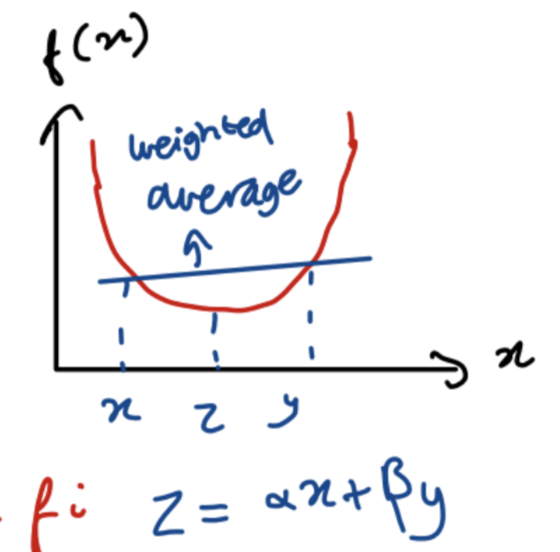
\includegraphics[width=0.2\linewidth]{Screenshot 2023-01-23 at 17.04.34.png}
\end{figure}
Special cases are the least-squares + linear programming \\ 
There is no analytical solution, and the computational time is roughly proportional to $\max \{n^3,n^2m,F\}$ where F is the cost of evaluating $f_i$ and their first + second derivatives
\subsection{Quadratic Programming}
Special case of convex optimisation: Assume $P = P^T \geq 0$
\[
\centering
\begin{aligned}
\min_x 0.5x^T P x + q^T x + r \\ s.t \;  Gx \leq h \\ Ax = b
\end{aligned}
\]
\subsection{Optimisation in Control}
System: $x_{k+1} = f(x_k,u_k), \; y = h(x_k,u_k)$, input u, state x, output y \\ 
Example optimal solutions:
\begin{itemize}
    \item Drive the system optimally:
    \begin{itemize}
        \item Find the optimal sequence $u_k^*$ - could minimise energy/time
        \item Find the optimal trajectory $x_k^*$ - shortest path
    \end{itemize}
    \item Optimal feedback control
    \begin{itemize}
        \item Find state-feedback controllers: $u = \sum x$ (complete information) or output feedback controllers $u = \sum y$ (incomplete information) which guarantee optimal closed loop performance/robustness
        \item Optimisation assisted control
        \begin{itemize}
            \item Predictive control (handling constraints)
            \item Controllers that learn
            \item Computer-assisted control design
        \end{itemize}
    \end{itemize}
\end{itemize}
\section{Optimal Control and Dynamic Programming}
\subsection{Discrete-time Optimal Control}
\subsubsection*{States and Inputs}
\begin{itemize}
    \item State $x \in X$ e.g $X = \mathbb{R}^n$
    \item Input $u \in U$ e.g $U = \mathbb{R}^m$
\end{itemize}
\subsubsection*{Dynamics}
Discrete-time state space system: $x_{k+1} = f(x_k,u_k)$, where $f(\cdot, \cdot) : X \times U \rightarrow X$ \\ We assume that the initial condition $x_0$ is given.
\subsubsection*{Trajectory}
Given $x_0$ each input sequence $u_0,...,u_{h-1}$ generates a state sequence $x_0,...,x_h$ such that $x_{k+1} = f(x_k,u_k)$ for $k=0,\hdots, h-1$
\subsubsection*{Finite Horizon Cost Function}
\[
J(x_0, u_0,...,u_h-1) = \sum_{k=0}^{h-1} c(x_k,u_k) + J_h(x_h)
\]
Where $\sum_{k=0}^{h-1} c(x_k,u_k)$ is the stage cost and $J_h(x_h)$ is the terminal cost \\
We then want to find the best input sequence $u_0^*,...,u_{h-1}^*$ such that: 
\[
J^*(x_0) = \min_{u_0,...,u_{h-1}} J(x_0,u_0,...,u_{h-1})
\]
Note that: $J^*$ might not be well-defined, and $u_0^*,..u_{h-1}^*$ might not exist or be non-unique
\subsubsection*{Bellman's Principle of Optimality}
We can truncate the original problem to form:
\[
\min_{u_k,...,u_{h-1}} \left(\sum_{i=k}^{h-1} c(x_i,u_i) + J_h(x_h) \right)
\]
To solve this, the solution can be defined as $V(\cdot, \cdot) : X \times \{0,...,h\} \rightarrow \mathbb{R}$. Then:
\[
V(x,k) \triangleq \min_{u_k,...,u_{h-1}} \left( \sum_{i=k}^{h-1} c(x_i,u_i) + J_h(x_h) \right)
\]
In this instance V(x,k) is the value function/cost to go. This is the optimal additional cost from the kth step on. \\ If we know V(x,k+1) for all x, then we can rewrite V(x,k) as:
\[
\begin{aligned}
V(x,k) &= \min_{u_k,...,u_{h-1}} \left( \sum_{i=k}^{h-1} c(x_i,u_i) + J_h(x_h) \right) \\ &= \min_{u_k,...,u_{h-1}} \left( c(x_k,u_k) + \sum_{i=k+1}^{h-1} c(x_i,u_i) + J_h(x_h) \right) \\ &= \min_{u_k} \left( \min_{u_k,...,u_{h-1}} \left( c(x,u_k) + \sum_{i=k+1}^{h-1} c(x_i,u_i) + J_h(x_h)\right)  \right) \\
&= \min_{u_k} \left( c(x,u_k) + \min_{u_k,...,u_{h-1}} \left( \sum_{i=k+1}^{h-1} c(x_i,u_i) + J_h(x_h) \right) \right)
\\ 
&= \min_{u_k} \left( c(x,u_k) + V(x_{k+1},k+1) \right)
\end{aligned}
\]
Thus we have recursion to express V(x,k) in terms of V(x,k+1) \\ \\
Hence we can find the optimal cost and optimal control by solving the dynamic programming equation: 
\begin{equation}\label{dp1}
V(x,k) = \min_u (c(x,u) + V(f(x,u),k+1)), \; k=h-1,h-2,...1,0
\end{equation}
With the final condition: $V(x,h) = J_h(x)$

The optimal cost can then be found by:
\[
J^*(x_0) = \min_{u_0,...,u_{h-1}} J(x_0,u_0,...,u_{h-1}) = V(x_0,0)
\]
The optimal input $u_k$ at each step minimises Equation \eqref{dp1} for the current value of state $x_k$. We can also define 
\[
g(x,k) = \operatorname*{argmin}_u (c(x,u) + V(f(x,u),k+1))
\]
The optimal control would then be:
\[
u_k^* = g(x_k,k) \; k=0,1,...,h-1
\]
Note that:
\begin{itemize}
    \item arg min is the value which achieves the minimum
    \item This converts the minimisation over a sequence of h inputs to a sequence of h minimisations over 1 input, but all states
    \item Optimal controls are given by time varying state feedback
    \item Solution has been computed all for $x_0$
    \item If the state and input can only take a finite number of values, then the optimisation can be performed by enumeration
\end{itemize}
\subsubsection*{Example}
\begin{figure}[H]
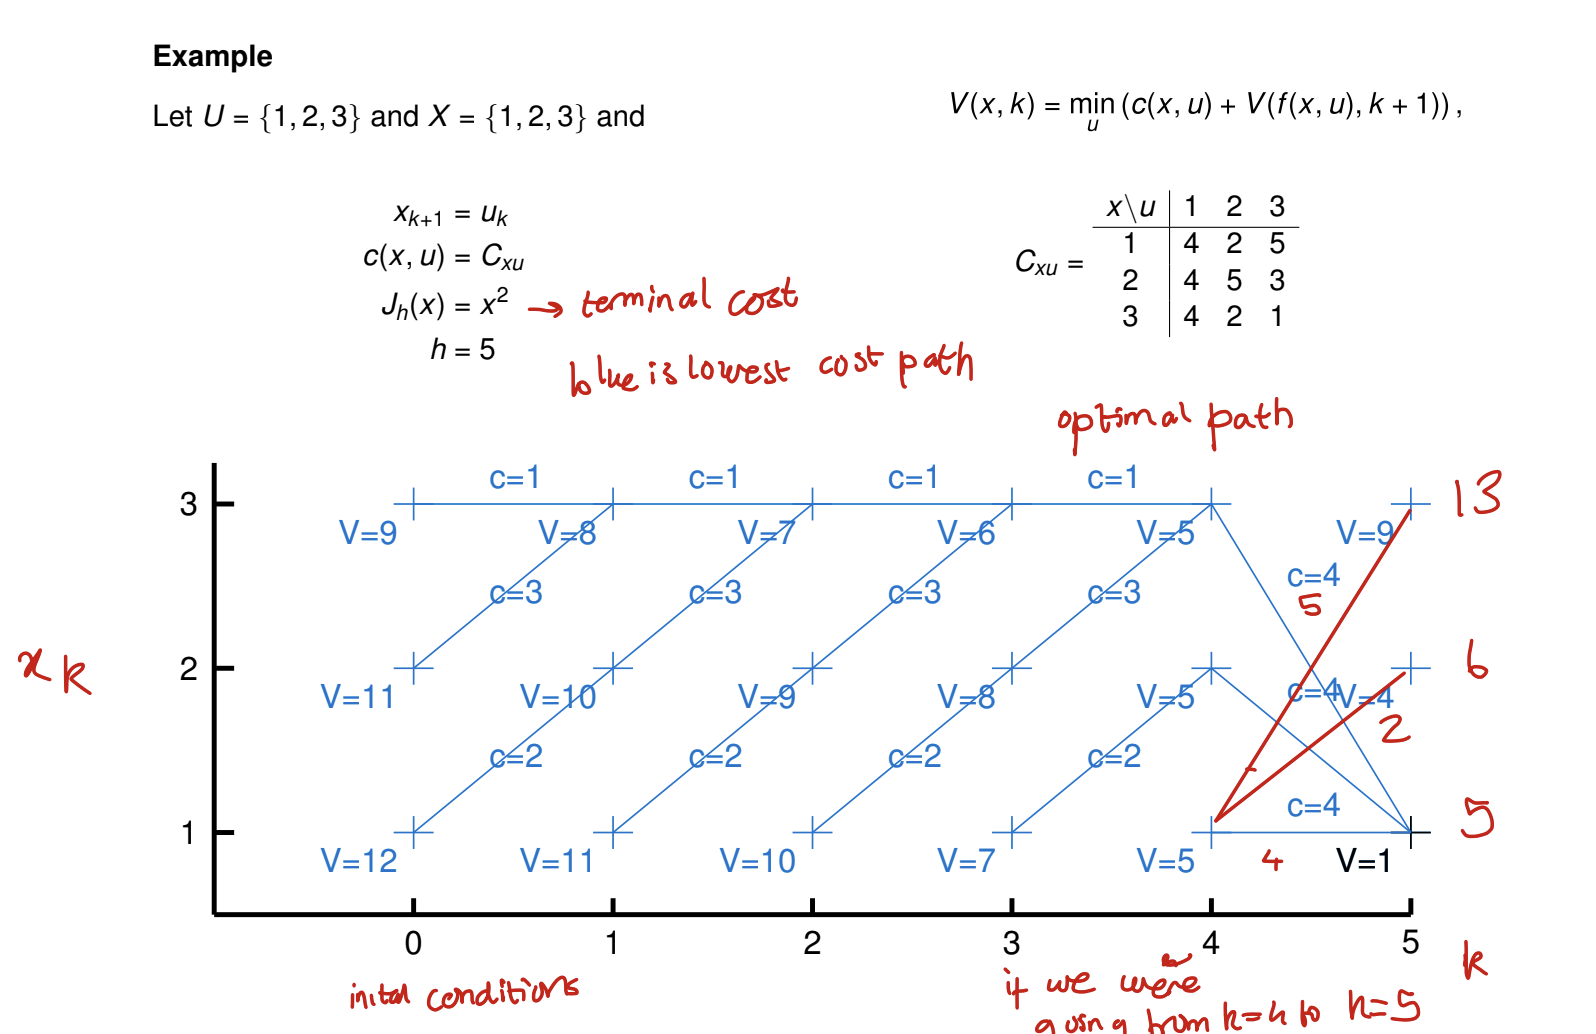
\includegraphics[width = \linewidth]{example1.png}
\end{figure}
Looking at the possible options from k=4 to k=5, where the current state is $x_k = 1$:
\begin{itemize}
    \item With an input of $u_k = 1$, then $x_{k+1} = 1$, the cost is $C_{11} = 4$, and the total cost is $4 + J_h(1) = 5$
    \item With an input of $u_k = 2$, then $x_{k+1} = 2$, and the total cost is $C_{12} + J_h(2) = 6$
    \item With an input of $u_k = 3$, then $x_{k+1} = 3$, the total cost is $C_{13} + J_h(3) = 13$
\end{itemize}
Thus the optimal path from $x_4=1$ to $x_5$ is with input $u_k = 1$.
This is repeated for the other possible paths.
\subsection{Discrete-time Linear Quadratic Regulator (LQR)}
\subsubsection*{States and Inputs}
State $x \in X = \mathbb{R}^N$, Input $u \in U = \mathbb{R}^m$
\\ 
\subsubsection*{Dynamics}
$x_{k+1} = A x_k + B u_k$, where we assume that the initial condition $x_0$ is given
\subsubsection*{Cost Function}
We can then define the cost function as:
\[
\centering
J(x_0,u_0,u_1,...,u_{h-1}) = \sum_{k=0}^{h-1} \left( x_k^T Q x_k + u_k^T R u_k \right) + x_h^T X_h x_h 
\]
Where Q,R, $X_h$ are symmetric matrices with Q $\geq$ 0, R > 0, $X_h \geq 0$. For a matrix to be greater than 0, then $x^T A x > 0$ for all x $\neq$ 0, and hence an inverse exists for that matrix.
\begin{lemma}{(Minimisation for Quadratic Forms)}\label{lma1}
\\ \\ 
For symmetric matrices Q, R, for R > 0, then:
\[
\begin{aligned}
\min_u \begin{bmatrix}
x^T & u^T
\end{bmatrix}
\begin{bmatrix}
Q & S^T \\ S & R
\end{bmatrix}
\begin{bmatrix}
x \\ u
\end{bmatrix}
= x^T(Q - S^T R^{-1} S) x 
\end{aligned}
\]
This minimum is achieved when:
\[
u = -R^{-1}Sx
\]
We can prove this by completing the square:
\[
\begin{aligned}
\begin{bmatrix}
x^T & u^T
\end{bmatrix}
\begin{bmatrix}
Q & S^T \\ S & R
\end{bmatrix}
\begin{bmatrix}
x \\ u
\end{bmatrix}
&= \begin{bmatrix}
(x^T Q + u^T S) & (x^T S^T + u^T R) 
\end{bmatrix}
\begin{bmatrix}
    x \\ u
\end{bmatrix}
\\ 
&= x^T Q x + u^T S x + x^T S^T u + u^T R u \\ 
&= (u^T + x^T S^T R^{-1})R(u + R^{-1}Sx) + x^T Q x - x^T S^T R^{-1}Sx \\
&\begin{cases}
= x^T(Q - S^T R^{-1}S)x & \text{ \normalfont if } u= -R^{-1}Sx \\
\geq x^T(Q - S^T R^{-1}S) x & \text{ \normalfont for all u, as the brackets term is positive since R is positive definite}
\end{cases}
\end{aligned}
\]
This can also be proved by matrix calculus
\[
\begin{aligned}
\begin{bmatrix}
x^T & u^T
\end{bmatrix}
\begin{bmatrix}
Q & S^T \\ S & R
\end{bmatrix}
\begin{bmatrix}
x \\ u
\end{bmatrix}
&= \begin{bmatrix}
(x^T Q + u^T S) & (x^T S^T + u^T R) 
\end{bmatrix}
\begin{bmatrix}
    x \\ u
\end{bmatrix}
\\ 
&= x^T Q x + u^T S x + x^T S^T u + u^T R u
\end{aligned}
\]
\begin{itemize}
    \item\text{ \normalfont There is a stationary point here when $\nabla_u = (x^T Q x + u^T S x + x^T S^T u + u^T R u) = 0$}
    \item\text{ \normalfont At the stationary point $2 (Sx + Ru) = 0 \implies u = R^{-1}Sx$
}
    \item\text{ \normalfont
We can check this is a minimum as: $\nabla_u^2 (x^T Q x + u^T S x + x^T S^T u + u^T R u) = 2R > 0$ 
    }
\end{itemize}
\end{lemma}
Thus, the dynamic programming equation \eqref{dp1} can be simplified to:
\[
V(x,k) = \min_u \left( \underbrace{x^T Qx + u^T R u}_{c(x,u)} + V (\overbrace{Ax + Bu, k+1}^{f(x,u)})  \right)
\]
To use this equation, we can look at the penultimate time step h-1, since we know the value function at time step h $\rightarrow$ the terminal cost:
\[
\begin{aligned}
V(x,h-1) &= \min_u \left( x^T Q x + u^T R u + \overbrace{\underbrace{(Ax + Bu)^T}_{X_h^T} X_h \underbrace{(Ax + Bu)}_{X_h}}^{J_x(x_h)} \right) \\ 
&= \min_u \begin{bmatrix}
    x^T & u^T
\end{bmatrix}
\begin{bmatrix}
    Q + A^T X_h A & A^T X_h B \\ B^T X_h A & R + B^TX_h B 
\end{bmatrix}
\begin{bmatrix}
    x \\ u
\end{bmatrix}
\end{aligned}
\]
This form is similar to \eqref{lma1}, and thus we can solve this:
\[
\begin{aligned}
\tilde{Q} &= Q + A^T X_h A, \; \; \tilde{S} = B^T X_h A, \\ \tilde{R} &= R + B^TX_h B,  \; \; u = -\tilde{R}^{-1} \tilde{S} x
\\ 
V(x,h-1) &= x^T \underbrace{(Q + A^T X_h A - A^T X_h B (R + B^T X_h B)^{-1} B^T X_h A)}_{X_{h-1}} x 
\end{aligned}
\]
Thus, we can solve the problem recursively:
\[
\begin{aligned}
    V(x,h) &= x^T X_h x \\
    V(x,h-1) &= x^T X_{h-1}x \\
    \vdots \\ 
    V(x,0) &= x^TX_0 x
\end{aligned}
\]
\\
\begin{lemma}{ \normalfont Matrix $X_k \geq 0,k=h,h-1,...,0$ \normalfont if $X_h \geq 0, Q \geq 0, R > 0$}\label{lma2}
\\  \\ 
Proof:
\[
X_{h-1} = Q + A^T(X_h - X_hB(R + B^T X_h B)^{-1} B^T X_h)A
\]
\text{\normalfont For this, it is sufficient to have $ Q \geq 0$ and $X_h - X_hB(R + B^TX_hB)^{-1} B^T X_h \geq 0$}
\\ \\
\text{\normalfont Let $M = (B^TX_h B + R)$}

\begin{gather*}
\begin{bmatrix}
I && B^T
\end{bmatrix}
X_h
\begin{bmatrix}
    I & B
\end{bmatrix}
\geq 0, \; \; 
\begin{bmatrix}
    0 & 0 \\ 0 & R
\end{bmatrix}
\geq 0 \implies \begin{bmatrix}
    X_h & X_h B \\ B^T X_h & (B^TX_h B + R)
\end{bmatrix} 
\geq 0
\\
\begin{bmatrix}
    I & -X_hBM^{-1} \\ 0 & I
\end{bmatrix}
\begin{bmatrix}
    X_h & X_hB \\ B^TX_h & M 
\end{bmatrix}
\begin{bmatrix}
    I & 0 \\ -M^{-1}B^TX_h & I 
\end{bmatrix}
\geq 0 
\\ 
\begin{bmatrix}
    X_h - X_h BM^{-1}B^TX_h & 0 \\ 0 & M
\end{bmatrix}
\geq 0
\end{gather*}
\text{\normalfont As this is a diagonal element, then the individual elements must be greater than 0, so the lemma is proved}
\end{lemma}
Overall, to solve the LQR, we need to solve the backwards difference equation:
\[
X_{k-1} = Q + A^T X_k A - A^T X_kB(R + B^TX_k B)^{-1} B^T X_k A
\]
This has an optimal cost of:
\[
x_0^TX_0x_0
\]
when there is a state-feedback control of:
\[
u_k = -(R + B^T X_{k+1}B)^{-1}B^TX_{k+1}Ax_k
\]
\subsection{Continuous-Time Dynamic Programming}
\subsubsection*{States and Inputs}
$x \in \mathbb{R}^n$, $u \in U \subseteq \mathbb{R}^m $, e.g $U = [-1,1]$
\subsubsection*{Dynamics}
In this case, it is a continuous-time state space system:
\[
\dot x = f(x,u), \; f(\cdot, \cdot) : \mathbb{R}^n \times U \rightarrow \mathbb{R}^n
\]
For example, $\dot x = sin(x) + u$
\subsubsection*{Trajectory}
With a initial state $x_0 \in X$, and a horizon $T \geq 0$, then each input function $u (\cdot) : [0,T] \rightarrow U$ will produce a state trajectory $x(\cdot) : [0,T] \rightarrow \mathbb{R}^n $, where $x(0) = x_0, \; \dot x(t) = f(x(t),u(t))$
\subsubsection*{Cost Function}
\[
J(x_0,u( \cdot)) = \int_0^T c(x(t),u(t)) dt + J_T(x(T))
\]
\subsubsection*{Objective}
We want to find the best input function $u^*(\cdot) : [0,T] \rightarrow U$ which minimises the cost function:
\[
J^*(x_0) = J(x_0,u^*(\cdot)) = \min_{u (\cdot)} J(x_0,u(\cdot))
\]
Note that we assume that a unique trajectory exists for each state, and that we can find the minimum cost and input for our problem
\subsubsection*{Bellman's Principle of Optimality}
Again, Bellman's principle can apply here. If we assume that the optimal control $u^*(\cdot) : [0,T] \rightarrow U$ gets us from $x(0) = x_0$ to $x(t)$ at time t < T. Then again, the problem can be truncated to show that $u^*(\cdot) : [t,T] \rightarrow U$ is a solution to:
\[
\min_{u (\cdot)} \int_t^T c(x(\tau),u(\tau)) d \tau + J_T(x(T))
\]
\subsubsection*{Solution}
We can define a value function/cost to go again $V : X \times [0,T] \rightarrow \mathbb{R}$:
\[
V(x(t),t) \triangleq \min_{u (\cdot)} \int_t^T c(x(\tau),u(\tau)) d \tau + J_T (x(T))
\]
In this case, we know that $V(x(T),T) = J_T(x(T))$ is the final cost, and $V(x(0),0) = J^*(x(0))$ is the optimal cost from the initial condition $x(0)$.
\\
To find the optimal solution, consider an infinitesimal time later h. Then Bellman's Equation becomes:
\[
\begin{aligned}
V(x(t),t) &= \min_{u(\cdot)} \int_t^{t+h} c(x(\tau), u(\tau)) d\tau + \int_{t+h}^T c(x(\tau),u(\tau)) d\tau + J_T(x(T))
\\
&= \min_{u(\cdot)} \int_t^{t+h} c(x(\tau), u(\tau)) d\tau + V(x(t+h),t+h)
\end{aligned}
\]
\\
From here, we can consider sampling at every h time step. Thus:
\[
x(t+h) = x(t) + \underbrace{f(x(t),u(t))}_{\dot x} h + \mathcal{O}(h^2)
\]
The infinitesimal cost between t and t+h is then:
\[
\int_t^{t+h} c(x(\tau), u(\tau)) d\tau = c(x(t),u(t))h + \mathcal{O}(h^2)
\]
Hence, the dynamic programming equation can be approximated as:
\[
V(x,t) = \min_{u \in U} (c(x,u)h + V(x + f(x,u)h, t+h)) + \mathcal{O}(h^2)
\]
With a terminal cost of $V(x,T) = J_T(x)$. \\
To solve this, we can consider the Taylor series expansion:
\[
V(x + \delta x, t + \delta t) = V(x,t) + \frac{\partial V}{\partial x} \delta x + \frac{\partial V}{\partial t} \delta t + \mathcal{O}(\delta x^2, \delta t^2)
\]
Subbing this back into the earlier equation produces:
\[
\begin{aligned}
    V(x,t) &= \min_{u \in U} (c(x,u)h + V(x + f(x,u)h, t+h)) + \mathcal{O}(h^2) \\
    &= \min_{u \in U} \left( c(x,u)h + V(x,t) + \frac{\partial V(x,t)}{\partial x} f(x,u)h + \frac{\partial V(x,t)}{\partial t} h \right) + \mathcal{O}(h^2) \\ 
    V(x,t) - V(x,t) - \frac{\partial V(x,t)}{\partial x}h &= \min_{u \in U} \left( c(x,u)h  + \frac{\partial V(x,t)}{\partial x} f(x,u)h  \right) + \mathcal{O}(h^2) \\
    - \frac{\partial V(x,t)}{\partial x} &= \min_{u \in U} \left( c(x,u)  + \frac{\partial V(x,t)}{\partial x} f(x,u)  \right) + \frac{\mathcal{O}(h^2)}{h}
    \\
    \end{aligned}
\]
\text{Take the limit as $h \rightarrow 0$:} 
\begin{equation}\label{hjb}
    - \frac{\partial V(x,t)}{\partial x} = \min_{u \in U} \left( c(x,u)  + \frac{\partial V(x,t)}{\partial x} f(x,u)  \right)
    \end{equation}

This PDE can be used to find the value function, with boundary condition $V(x,T) = J_T(x)$. The optimal cost is $V(x_0,0)$ and the optimal input is:
\[
\begin{aligned}
    u^*(t) = g(x(t),t)  \\
    g(x,t) = \operatorname*{argmin}_{u \in U} \left( c(x,u)  + \frac{\partial V(x,t)}{\partial x} f(x,u)  \right)
\end{aligned}
\]
This equation \eqref{hjb} is known as the Hamilton-Jacobi-Bellman PDE. It is the infinitesimal version of \eqref{dp1}. It is much simpler to solve, as it turns the optimisation over $u(\cdot)$ which is a continuous function with infinite points as continuous time, into a pointwise optimisation over $u \in U$. \\
Note that in some cases, a solution might not exist, and even if it does exist it might not be able to be computed or make sense physically.
\subsection{Continuous-Time Linear Quadratic Regulator}
\subsubsection*{States and Inputs}
States $x \in \mathbb{R}^n$, Inputs $u \in \mathbb{R}^m$
\subsubsection*{Plant}
$\dot x = Ax + Bu, \; x(0) = x_0$
\subsubsection*{Cost Function}
\[
\begin{aligned}
    J(x_0,u(\cdot)) &= \int_0^{t_1} c(x,u)dt + J_{t_1} (x(T)) \\
    c(x,u) &= x^T Qx + u^T R u \\
    R &= R^T > 0 \\
    X_{t_1} &= X_{t_1}^T \geq 0 \\
    J_{t_1}(x) &= x^T X_{t_1}x \\ 
    Q &= Q^T \geq 0
\end{aligned}
\]
To solve this, we use the HJB Equation \eqref{hjb}:
\[
\begin{aligned}
    - \frac{\partial V(x,t)}{\partial x} = \min_{u \in U} \left( c(x,u)  + \frac{\partial V(x,t)}{\partial x} f(x,u)  \right)
\end{aligned}
\]
Subbing in for the $c(x,u), f(x,u)$ shows that:
\[
\begin{aligned}
    c(x,u) = x^T Q x + u^T R u, f(x,u) &= Ax + Bu \\
    \text{Guess a solution: } V(x,t) &= x^T X(t)x \\
    -x^T \dot X(t) x &= \min_{u \in \mathbb{R}^m} \left( x^T Q x + u^T R u + 2 x^T X(t)(Ax + Bu) \right) \\
    &= \min_{u \in \mathbb{R}^m} \left( x^T(Q + XA + A^T X) + u^T R u + x^T XBu + u^T B^T Xx \right) \\
    &= x^T(Q + XA + A^T X - XBR^{-1}B^T X)x \\
    u^*(t) &= -R^{-1}B^T X(t) x(t)
\end{aligned}
\]
Essentially, this is solving the ODE (Riccati Equation): 
\[
\begin{aligned}
    - \dot X &= Q + XA + A^T X - XBR^{-1}B^T X \\
    X(t_1) &= X_{t_1}
\end{aligned}
\]
The optimal cost is given by $x_0^T X(0) x_0$, and the optimal input is $u(t) = -R^{-1} B^T X(t) x(t)$. \\
To do the backwards numerical integration, we can use that:
\[
\begin{aligned}
    \dot X (t) &\simeq \frac{X(t) - X(t-\Delta t)}{\Delta t}\\
    X(t - \Delta t) &\simeq X(t) - \dot X(t) \Delta t \\
    &\simeq X(t) + (Q + X(t) A + A^T X(t) - X(t) BR^{-1}B^T X(t)) \Delta t
\end{aligned}
\]
\subsubsection*{Example: Minimum energy input to reach a state}
Consider a cost:
\[
J(\tilde{x}(0),u(\cdot)) = \int_0^{t_1} \tilde u(t)^T \tilde u(t) dt + \frac{1}{\epsilon} \tilde x(t_1)^T \tilde x(t_1)
\]
Where $\tilde x = x_1 - x$ and $\tilde u = u_1 - u$. Essentially $x_1,u_1$ is a fixed point, which could be equilibrium i.e $Ax_1 + B u_1 = 0$. In this case $c(\tilde x, \tilde u) = \tilde u^T \tilde u$, Q = 0, R = I. \\
To do this, we solve the Riccati Equation: 
\[
\dot X = Q + XA +A^T X - XBR^{-1}B^T X = XA + A^T X - XBB^TX 
\]
Where the terminal condition X(T) = $\frac{1}{\epsilon}$ I. The optimal input would again be:
\[
\tilde u^*(t) = -B^T X(t) \tilde x(t)
\]
As $\epsilon \rightarrow 0$ and $\tilde x(0) = x_1, u = \tilde u^*(\cdot) + u_1$. u is the minimum energy input to drive the state from $x(0) = 0$ to $x(t_1) = x_1$. \\
Consider again the Riccati Equation:
\[
-\dot X = XA + A^TX - XBB^T X
\]
To solve this, we can use the substitution $Y = -X^{-1}$. \\ Note that: $\frac{d}{dt} Y^{-1} = - Y^{-1} \dot Y Y^{-1}$. Then we get that:
\[
-Y^{-1}\dot Y Y^{-1} = -Y^{-1}A - A^T Y^{-1} - Y^{-1}BB^T Y^{-1}
\]
The optimal control in this case would satisfy:
\[
u^*(t) = B^TY^{-1}(t) \tilde x(t) \; \; \; (\tilde x(0) = x_1)
\]
where:
\[
\dot Y = AY + YA^T + BB^T
\]
and $Y(t_1) = \epsilon I$ (this is the Lyapunov equation - easier to solve and integrate)
\subsection{Infinite Horizon Linear Quadratic Regulator - continuous case}
\subsubsection*{Plant}
$\dot x = Ax + Bu$, $x(0) = x_0$, $z = \begin{bmatrix}
    Cx \\ u
\end{bmatrix}$
\subsubsection*{Cost Function}
\[
\begin{aligned}
    J(x_0,u(\cdot)) &= \int_0^\infty z(t)^T z(t) dt \\
    &= \int_0^\infty \left( \underbrace{x(t)^T C^T C x(t)}_{\text{output energy}} 
    + \underbrace{u(t)^T R u(t)}_{\text{input energy, R = I}} \right) dt
\end{aligned}
\]
\subsubsection*{Assumptions}
(A,B) controllable, (A,C) observable 
\subsubsection*{Solution}
We can assume that an infinite horizon is a finite but very long horizon 
\[
\lim_{t_1 \rightarrow \infty} \int_0^{t_1} x(t)^T C^T C x(t) + u(t) R u(t) dt
\]
Therefore, we can find the solution from the Riccati equation:
\[
-\dot X(t) = C^TC + X(t) A + A^T X(t) - X(t) BRB^T X(t)
\]
where there can be any final condition $X(t_1) = X^T(t_1) > 0$
\subsubsection*{Solution}
We can guess that the solution will be of the form $u(t) = -B^T X x(t)$, where $X = X^T$ solves the Control Algebraic Riccati Equation (CARE):
\begin{equation}\label{care}
0 = C^TC + XA + ATX - XBB^T X 
\end{equation}
The closed-loop dynamics would be controlled by:
\[
\dot x = Ax + Bu = (A-BB^T X)x
\]
and we would want $(A-BB^TX)$ is stable (all eigenvalues in left-half plane)
\subsubsection*{Fact}
Based on the earlier assumptions, the CARE \eqref{care} has a unique, symmetric, positive,definite solution $X = X^T > 0$, which is stabilising ($(A-BB^TX)$ is stable). We can also obtain this solution from $\lim_{t \rightarrow -\infty} X(t)$, where $X(t)$ solves:
\[
-\dot X(t) = C^TC + X(t) A + A^T X(t) - X(t) BB^T X(t)
\]
This is essentially solving backwards in time. This case applies for any final condition $X(T) = X^T(T) > 0$
\subsubsection*{Summary}
Let $X = X^T$ be the stabilising solution to CARE \eqref{care}. Then the optimal control is given by $u(t) = -B^T Xx(t)$, and the optimal cost is $x(0)^T X x(0)$
\subsection{Infinite Horizon Linear Quadratic Regulator - Discrete Case}
\subsubsection*{Plant}
$x_{k+1} = Ax_k + Bu_k$, $x(0) = x_0$, $z = \begin{bmatrix}
    Cx \\ u
\end{bmatrix}$ 
\subsubsection*{Cost Function}
\[
J(x_0,u_0,u_1,...) = \sum_{k=0}^{\infty} x_k^T Q x_k + u_k^T R u_k
\]
\subsubsection*{Assumptions}
(A,B) controllable, (A,Q) observable
\subsubsection*{Solution}
Again, think of an infinite horizon as a very long finite horizon. Using previous results, the optimal state-feedback control is:
\[
u_k = -(R + B^T X B)^{-1} B^T XAx_k
\]
Where $X = X^T$ solves the Discrete Algebraic Riccati Equation
\begin{equation}\label{dare}
X = Q + A^TXA - A^TXB(R+B^TXB)^{-1}B^TXA
\end{equation}
for $X = X^T > 0$. The optimal cost is: 
\[
x_0^T X x_0
\]
\section{ \texorpdfstring{$\mathcal{H}_2 \; \text{norm}$}. }
\subsection{The \texorpdfstring{$\mathcal{H}_2 \; \text{norm}$} .}
Consider the stable linear system:
\[
\dot x = Ax + Bu, \; y = Cx
\]
Where A has all its eigenvalues in the left half plane. The system would then have a transfer function:
\[
G(s) = C(sI - A)^{-1} B
\]
Then the $\mathcal{H}_2$ norm is defined as:
\[
\begin{aligned}
    ||G||_2^2 &= \int_{-\infty}^\infty \text{trace}\{\bar{G(j\omega)}^T G(j\omega) \} d\omega \\
    ||G||_2^2 &= \sum_i ||G_i||_2^2
\end{aligned}
\]
Where $G_i$ is the transfer function from the ith input to the output i.e $G_i : T_{ui} \rightarrow y$. \\
Therefore, you can show that:
\[
\begin{aligned}
||y||_\infty &\leq \frac{1}{\sqrt{2 \pi}}||G||_2 ||u||_2 \\
||y||_\infty &= \sup_t \sqrt{y^T(t) y(t)} \\
||u||_2 &= \sqrt{\int_{-\infty}^\infty u^T(t) u(t) dt}
\end{aligned}
\]
Where sup is the smallest upper bound of a set. The aim of $\mathcal{H}_2$ optimal control is to minimise the $\mathcal{H}_2$ norm of a closed-loop transfer function. \\ 
Let the impulse response of G(s) be g(t). As $G(s) = C(sI-A)^{-1} B$, and $g(t) = \mathcal{L}^{-1} G(s) = Ce^{At} B$. \\
From Parseval's Theorem, we know that: 
\[
\frac{1}{\sqrt{2\pi}} ||G(s)||_2 = ||g(t)||_2, \; ||g(t)||_2^2 = \sum_i ||g_i(t)||_2^2
\]
$g_i(t)$ is the response to an impulse on the ith input with $x(0^{-}) = 0$. \\ 
Hence,  $g_i(t) = 0$ for t < 0, but for $t \geq 0$ it is equal to the response of the system where: 
\[ x(0^+) = B_i \]
the ith column of B. This works if we compare the initial response: $Ce^{At} x_0$, to the general response: $Ce^{At} B$, under input u=0. \\
Then the problem is now computing the response of the system under u=0 starting at the appropriate initial conditions $x(0) = x_0$. \\
Consider the function $V(t) = x(t)^T L x(t), L = L^T$. If u = 0, then: \[ \begin{aligned}
\dot V(t) + y(t)^T y(t) &= \frac{d}{dt} (x(t)^T L x(t)) + y(t)^T y(t) \\
&= (Ax(t))^T L x(t) + x(t)^T LAx(t) + x(t)^T C^T C x(t) \\
&= x(t)^T (A^T L + LA + C^TC) x(t)
\end{aligned}
\]
If we choose $L = L^T >0$ to be the solution of the Lyapunov Equation:
\begin{equation}\label{lyapunov}
    A^T L + LA + C^TC = 0
\end{equation}
i.e L is the observability gramian, then the equation simplifies to:
\[
\dot V(t) + y(t)^T y(t) = 0
\]
If we integrate from 0 to $\infty$ then:
\[
[V(t)]_{0}^\infty + ||y||_2^2 = 0
\]
Since A is stable, and u= 0 then:
\[
\lim_{t \rightarrow \infty} x(t) = 0
\]
Therefore:
\[
\lim_{t \rightarrow \infty} V(t) = \lim_{t \rightarrow \infty} x^T (t) L x(t) = 0
\]
We also know that $V(0) = x_0^T L x_0$, so:
\[
||y||_2^2 = x_0^T L x_0
\]
So the response is also bounded. To find the impulse response for each input (i.e set $x_0 = B_i$: 
\[ 
\begin{aligned}
|| \tilde y_i ||_2^2 &= B_i^T L B_i \\
\sum_i || \tilde y_i(t)||_2^2 &= \sum_i (B_i^T L B_i) = \text{trace} (B^T L B)
\end{aligned}
\]
\subsubsection*{Summary}
\[
\frac{1}{\sqrt{2 \pi}} ||G(s)||_2 = \sqrt{\text{trace} (B^T L B)}, \; L = L^T
\]
This solves the Lyapunov equation \eqref{lyapunov}. We also know that: \[
\frac{1}{2 \pi} ||T_{u \rightarrow y}||_2^2 = \sum_i ||y(t)|_{u(t) = e_i \delta(t)}||_2^2
\]
and it can be shown that: 
\[
||y||_\infty = \sup_t \sqrt{y(t)^T y(t)} \leq \frac{1}{\sqrt{2 \pi}} ||T_{u \rightarrow y}||_2 ||u||_2
\]
\subsection{Linear Fractional Transformations}
\begin{figure}[H]
    \centering
    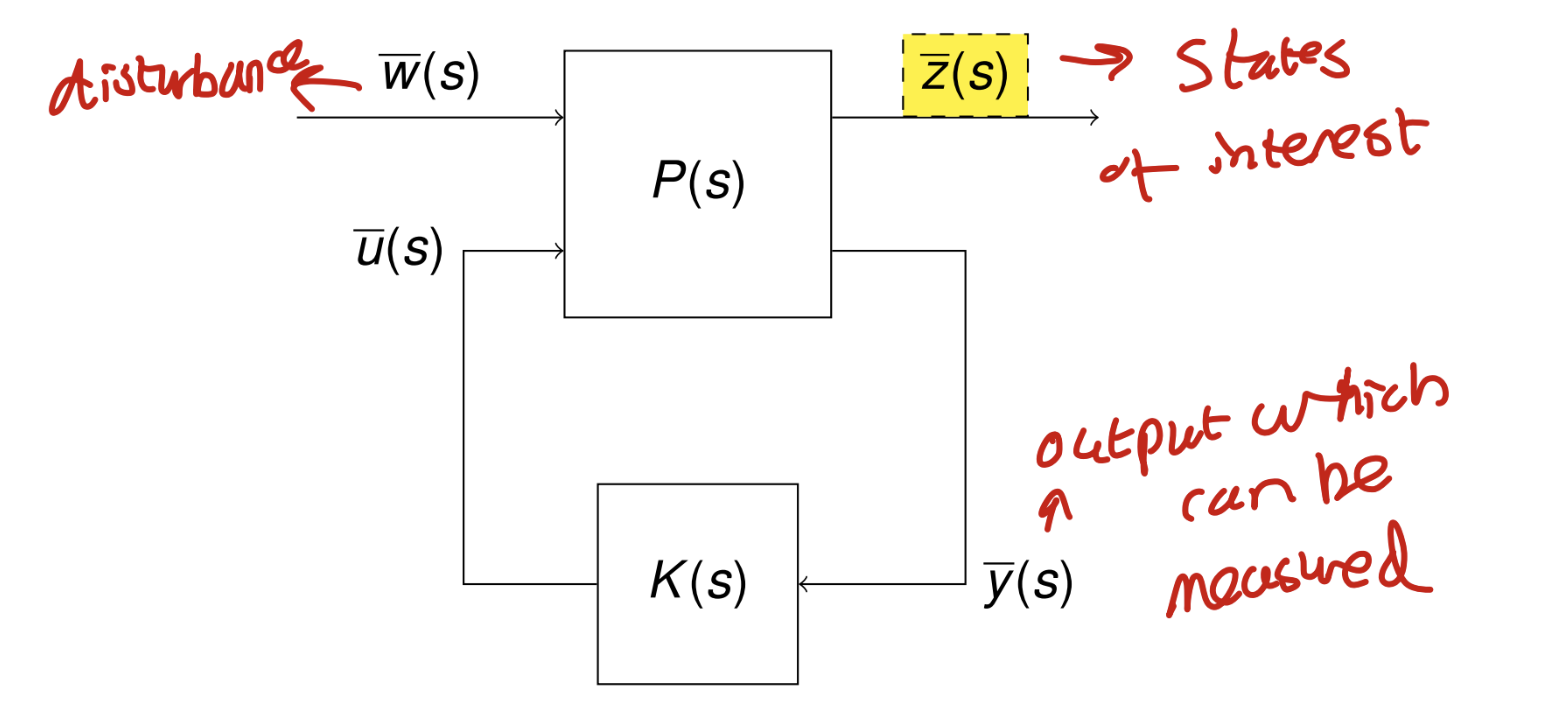
\includegraphics[width=0.6\linewidth]{Screenshot 2023-02-02 at 11.22.37.png}
\end{figure}
We can use Linear Fractional Transformations (LFTs) to manipulate closed-loop transfer functions. The lower LFT $\mathcal{F}_I(P(s),K(s))$ is the closed loop transfer function from $\bar w(s)$ to $\bar z(s)$ in this diagram. Hence:
\[
\mathcal{F}_I(P(s),K(s)) = T_{\bar w(s) \rightarrow \bar z(s)}
\]
In this case, P(s) is the Generalised Plant. \\
If P(s) has the block transfer representation:
\[
\begin{bmatrix}
    \bar z(s) \\ \bar y(s)
\end{bmatrix}
=
\underbrace{
\begin{bmatrix}
    P_{11}(s) & P_{22}(s) \\
    P_{21}(s) & P_{22}(s)
\end{bmatrix}}_{P(s)}
\begin{bmatrix}
    \bar w(s) \\ \bar u(s)
\end{bmatrix}
\]
Then we can obtain that:
\[
\begin{aligned}
    \bar z(s) &= P_{11}(s) \bar w(s) + P_{12}(s) \bar u(s) \\
    \bar y(s) &= P_{21}(s) \bar w(s) + P_{22}(s) \bar u(s) \\
    \bar u(s) &= K(s)\bar y(s) \\
    \bar u(s) &= K(s) ( P_{21}(s) \bar w + P_{22}(s) \bar u \\
    (1-KP_{22})\bar u &= KP_{21}\bar w \\
    \bar u &= (I - KP_{22})^{-1}KP_{21} \bar w \\
    \bar z &= P_{11} \bar w + P_{21} \bar u \\
    &= \left( P_{11} + P_{12}(I-KP_{22})^{-1} KP_{21}\right) \bar w \\
    &= \underbrace{\left(P_{11} + P_{21}K(I-KP_{22})^{-1}P_{21} \right)}_{\mathcal{F}_I (P(s),K(s))} \bar w
\end{aligned}
\]
Thus, the overall result is that:
\[
\bar z(s) = \mathcal{F}_I (P(s), K(s)) \bar w(s)
\]
Where
\[
\mathcal{F}_I(P(s),K(s)) = P_{11}(s) + P_{12}(s)K(s)(I-P_{22}(s)K(s))^{-1}P_{21}(s)
\]
We thus want to make $\mathcal{F}_I(P(s),K(s))$ small using stablising controllers $K(s)$ to reduce the $H_2$ norm of the system.
\subsection{\texorpdfstring{$\mathcal{H}_2$}. optimal control - state-feedback (a special case)}
If we let the generalised plant P have realisation
\[
\begin{aligned}
    \dot x &= Ax + B_1 w + B_2 u \\
    z &= \begin{bmatrix}
        C_1 x \\ u
    \end{bmatrix} \\
    y &= u \; \text{(state feedback)}
\end{aligned}
\]
This can be written in matrix form as:
\[
\begin{bmatrix}
    \dot x \\ z \\ y 
\end{bmatrix}
= \begin{bmatrix}
    A & B_1 & B_2 \\ \begin{bmatrix}
        C_1 \\ 0
    \end{bmatrix}
    & 0 &
    \begin{bmatrix}
        0 \\ I
    \end{bmatrix} \\
    I & 0 & 0
\end{bmatrix}
\begin{bmatrix}
    x \\ w \\ u
\end{bmatrix}
\]
Where we also assume that $(A,B_2)$ is controllable, and $(A,C_1)$ is observable.
\subsubsection*{Objective}
We want to find a K(s) which achieves:
\[
\min_{\text{K(s) stabilising}} = \underbrace{||\mathcal{F}_I (P(s),K(s))||_2^2}_{T_{w \rightarrow z}} = \min_{\text{K(s) stabilising}} 2 \pi \sum_i || z(t)|_{w(t) = e_i \delta(t)}||_2^2
\]
Where $e_i \delta(t)$, means that the state is applied at the ith input, so $e_i$ is:
\[
\begin{bmatrix}
    0 \\ \vdots  \\ 1 \\ \vdots \\ 0
\end{bmatrix}
\]
\subsubsection*{Solution}
From the LQR problem, we know that if $x(0)=x_0 \neq 0$, $w(t) = 0$, then:
\[
||z||_2^2 = x_0^TXx_0 + ||(u+B_2^TXx)||_2^2
\]
where $X = X^T$ is the stabilising solution to the CARE problem \eqref{care}
\[
0 = XA+A^TX +C_1^TC_1 - XB_2B_2^TX
\]
which is the unique solution for $A-B_2B_2^TX$ is stable. \\
If consider the situation where $x(0^{-1}) = 0$ and $w(t) = e_i \delta (t)$. This is equal to when $x(0^+) = B_1e_i, w(t) = 0$.  \\ Then:
\[
\left| \left| z(t)_{w(t) = e_i \delta(t)} \right| \right|_2^2 = e_i^TB_1^TXB_1e_i + \left| \left| (u+B_2^TXx)|_{x(0^+) = B_1 e_i} \right| \right|_2^2
\]
again $X=X^T$ is the stabilising solution of the same CARE. \\
If we define:
\[
v(t) = u(t) + B_2^T Xx(t)
\]
Then if $T_{w \rightarrow v}$ is the closed loop transfer function from w to v:
\[
\frac{1}{2\pi} ||T_{w \rightarrow v}||_2^2 = \sum_i ||v(t)_{w(t) = e_i \delta(t)}||_2^2 = \sum_i\left| \left| (u+B_2^TXx)|_{x(0^+) = B_1 e_i} \right| \right|_2^2
\]
Therefore:
\[
\frac{1}{2 \pi} ||\mathcal{F}_I(P(s),K(s))||_2^2 = \text{trace}(B_1^TXB_1) + \frac{1}{2 \pi}|| T_{w \rightarrow \underbrace{u + B_2^TXx}_{v}}||_2^2
\]
We can make $T_{w \rightarrow v} = 0$ by choosing 
\[
\bar u (s) = -B_2^T X \bar x(s)
\]
which is the same as choosing $K(s) = -B_2^T X$, where X is the solution of Riccati's equation \eqref{dare}
\subsubsection*{Summary}
\[
\min_{\text{K(s) stabilising}} ||\mathcal{F}_I(P(s),K(s))||_2 = \sqrt{2 \pi} \sqrt{\text{trace}(B_1^TXB_1)}
\]
Which is achieved by constant feedback gain $K = -B_2^TX$, and K(s) is stabilising by properties of CARE \eqref{care}
\subsection{\texorpdfstring{$\mathcal{H}_2$}. optimal control - output feedback}
For this, we don't know the full state vector x. Hence the generalised plant P is now:
\[
\begin{aligned}
\dot x &= Ax + B_1 w_1 + B_2 u_2 \\
z &= \begin{bmatrix}
    C_1 x \\ u
\end{bmatrix} \\
y &= C_2 x + w_2 \\ 
\begin{bmatrix}
    \dot x \\ z \\ y
\end{bmatrix}
&= \begin{bmatrix}
    A & \begin{bmatrix}
        B_1 & 0
    \end{bmatrix}
    & 
    B_2 \\
    \begin{bmatrix}
        C_1 \\ 0
    \end{bmatrix}
    & 0 & \begin{bmatrix}
        0 \\ I
    \end{bmatrix} \\
    C_2 & \begin{bmatrix}
        0 & I
    \end{bmatrix}
    & 0
\end{bmatrix}
\begin{bmatrix}
    x \\ w \\ u
\end{bmatrix}
\end{aligned}
\]
Where $w_1$ is the driving noise/disturbance, and $w_2$ is the observation noise. In this case $y \neq x$ as we don't know the exact feedback. \\
We can assume again that $(A,B_2)$ is controllable, and $(A,C_1)$ is observable. We can also assume that $(A,B_1)$ is controllable, and $(A,C_2)$ is observable for this estimation/dual problem. 
\subsubsection*{Solution}
Let $X = X^T$ be the stabilising solution ($A-B_2B_2^TX$) is stable for the care equation \eqref{care}. Then
\[
\frac{1}{2 \pi} ||\mathcal{F}_I(P(s),K(s))||_2^2 = \text{trace}(B_1^TXB_1) + \frac{1}{2 \pi}|| T_{w \rightarrow \underbrace{u + B_2^TXx}_{v}}||_2^2
\]
But we can't make $||T_{w \rightarrow v}||_2^2 = 0$ as we can't measure x. So instead, we can take $u = -B_2^T X x_k$, where $x_k$ is the estimation of x provided by an optimal observer. The optimal K would have the realisation
\[
\begin{aligned}
\begin{bmatrix}
    \dot x_k \\ u
\end{bmatrix}
= 
\begin{bmatrix}
    A-B_2F - HC_2 & H \\ -F & 0
\end{bmatrix}
\begin{bmatrix}
    x_k \\ y
\end{bmatrix} \\ 
F = B_2^TX, \; H = YC_2^T
\end{aligned}
\]
X and Y are the stabilising solution of:
\[
\begin{aligned}
    0 &= XA + A^T X + C_1^TC_1 - XB_2B_2^TX \; \textbf{(CARE)} \\
    0 &= YA^T + AY + B_1B_1^T - YC_2^TC_2Y \; \textbf{(FARE)}
\end{aligned}
\]
The optimal K would then achieve:
\[
\frac{1}{2 \pi} ||\mathcal{F}_I(P(s),K(s))||_2^2 =
\underbrace{\text{trace}(B_1^TXB_1)}_{\text{state f.b.}} + \underbrace{\text{trace}(FYF^T)}_{\text{output f.b. extra}} 
\]
\begin{figure}[H]
    \centering
    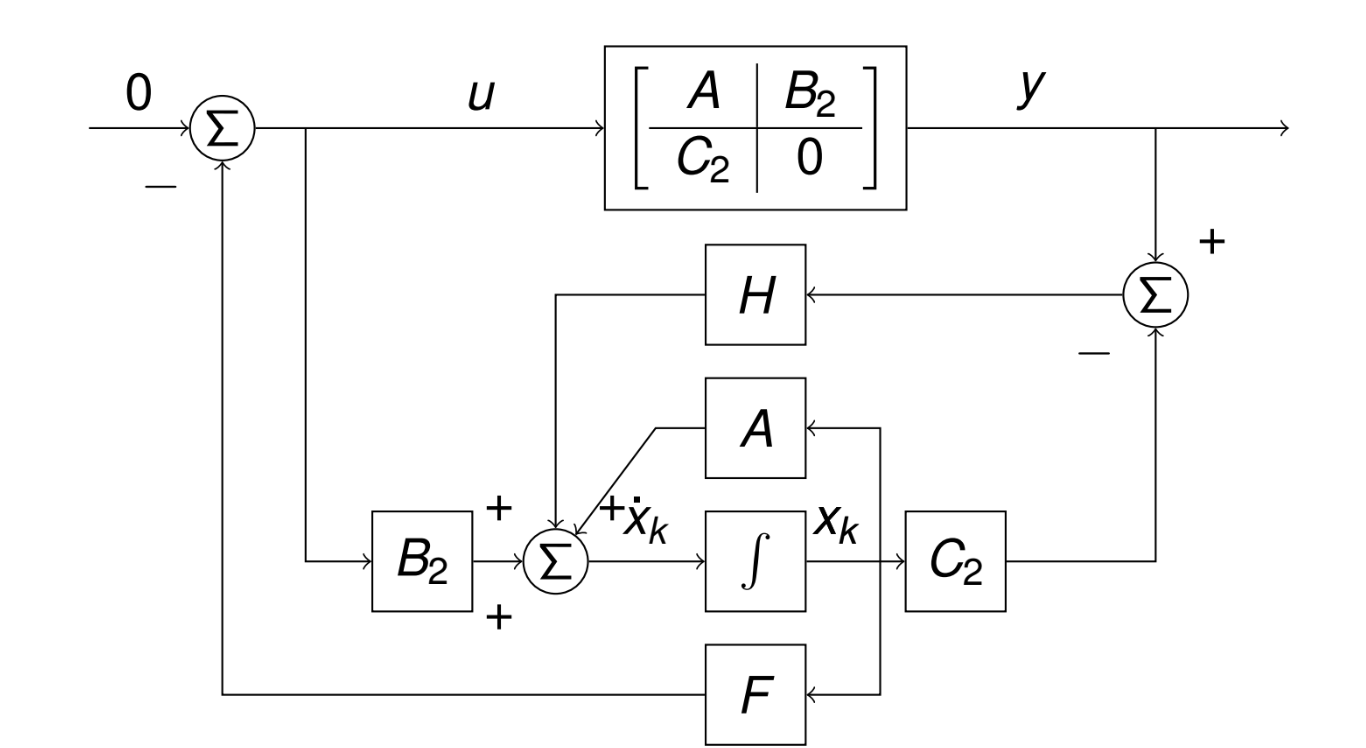
\includegraphics[width=0.6\linewidth]{Screenshot 2023-02-02 at 12.35.53.png}
\end{figure}
The closed loop poles of optimal K are: $\lambda_i(A-B_2F) \cup \lambda_i(A-HC_2)$, which are both stable
\subsubsection{\texorpdfstring{$\mathcal{H}_2$}. optimal control - output feedback (derivation)}
Note that:
\[
|| T_{w \rightarrow \underbrace{u + B_2^TXx}_{v}}||_2^2 = ||T_{w \rightarrow v}||_2^2 = ||\mathcal{F}_I (\tilde P,K)||_2^2
\]
where
\[
\begin{aligned}
\tilde P &= \begin{bmatrix}
    \dot x \\ z \\ y
\end{bmatrix}
 \begin{bmatrix}
    A & \begin{bmatrix}
        B_1 & 0
    \end{bmatrix}
    & 
    B_2 \\
    F
    & 0 & I \\
    C_2 & \begin{bmatrix}
        0 & I
    \end{bmatrix}
    & 0
\end{bmatrix}
\begin{bmatrix}
    x \\ w \\ u
\end{bmatrix} \\ 
F &= B_2^TX
\end{aligned}
\]
From there, since we know that $||G(s)||_2 = ||G(s)^T||_2$, then:
\[
\begin{aligned}
G(s) &= C(sI-A)^{-1}B + D, \\ G(s)^T &= B^T(sI-A^T)^{-1}C^T + D^T
\end{aligned}
\]
This can represented in matrix form:
\[
G(s) = \begin{bmatrix}
    A & B \\ C & D
\end{bmatrix}
\implies G(s)^T = \begin{bmatrix}
    A^T & C^T \\ B^T & D^T
\end{bmatrix}
\]
Furthermore
\[
\begin{aligned}
\mathcal{F}_I(\tilde P,K)^T &= \mathcal{F}_I(\tilde P^T,K^T) \\
(P_{11} + P_{12}K(I - P_{22}K)^{-1}P_{21})^T &= P_{11}^T + P_{21}^T(I-K^TP_{22}^T)^{-1}K^TP_{12}^T
\end{aligned}
\]
Using duality
\[
||\mathcal{F}_I(\tilde P,K)||_2 = ||\mathcal{F}_I(\tilde P^T,K^T)||_2
\]
Where $\tilde P^T$ has the realisation
\[
\begin{bmatrix}
     \tilde{\dot x} \\ \tilde z \\ \tilde y
\end{bmatrix}
 \begin{bmatrix}
    A^T & F^T
    & 
    C_2^T \\
    \begin{bmatrix}
        B_1^T \\ 0
    \end{bmatrix}
    & 0 & \begin{bmatrix}
        0 \\ I
    \end{bmatrix} \\
    B_2^T & I
    & 0
\end{bmatrix}
\begin{bmatrix}
    x \\ w \\ u
\end{bmatrix}
\]
Note that all the variables here e.g ($\tilde x$) are fictitious, not related to original variables. \\ \\
We can then apply state feedback results to get:
\[
\frac{1}{2 \pi} ||\mathcal{F}_I||_2^2 = \text{trace}(FYF^T) + \frac{1}{2 \pi} ||Y_{\tilde w \rightarrow \tilde u + C_2 Y \tilde x}||_2^2
\]
Where Y is the stabilising solution ($A - YC_2^TC_2$ is stable) to the Filter Algebraic Riccati Equation
\begin{equation}\label{fare}
    0 = YA^T + AY + B_1B_1^T - YC_2^TC_2Y
\end{equation}
From the earlier matrix, we know that:
\[
\begin{aligned}
\tilde{\dot x} &= A^T \tilde x + F^T \tilde w + C_2^T \tilde u  \\
\tilde y &= B_2^T \tilde x + \tilde w \\
\tilde{\dot x}_k &= A^T \tilde x_k + F^T \underbrace{( \tilde y - B_2^T \tilde x_k)}_{\tilde w} + C_2^T \tilde u
\end{aligned} 
\]
We can assume that $\tilde x_k(t) = \tilde x(t)$ for all t, so we can put that:
\[
\tilde u = -C_2 Y \tilde x_k = -H^T \tilde x_k
\]
Essentially, what we are saying is that we can measure the state at a certain time step k, and make that our desired state variables. \\
So the optimal K would have the realisation:
\[
\begin{bmatrix}
    \tilde{\dot x} k \\ u
\end{bmatrix}
= \begin{bmatrix}
    A^T - F^TB_2^T - C_2^TH^T & F^T \\
    -H^T & 0
\end{bmatrix}
\begin{bmatrix}
    \tilde x_k \\ \tilde y
\end{bmatrix}
\]
Then the original optimal K can be found by taking the transpose:
\[
\begin{bmatrix}
    \dot x_k \\ u
\end{bmatrix}
= \begin{bmatrix}
    A-B_2F - HC_2 & -H \\
    F & 0
\end{bmatrix}
\begin{bmatrix}
    x_k \\ y
\end{bmatrix}
\]
Where:
\[
F = B_2^TX, \; H = YC_2^T
\]
Where X and Y are the stabilising solution of CARE \eqref{care} and FARE \eqref{fare}.
\\
Another possible realisation of optimal K is:
\[
\begin{bmatrix}
    \dot x_k \\ u
\end{bmatrix}
= \begin{bmatrix}
    A-B_2F - HC_2 & H \\
    -F & 0
\end{bmatrix}
\begin{bmatrix}
    x_k \\ y
\end{bmatrix}
\]
This can be implemented in observer form.


\end{document}
